\documentclass{article}
\usepackage[utf8]{inputenc}
\usepackage[T1]{fontenc}
\usepackage{graphicx}
\usepackage{hyperref}
\usepackage{geometry}
\geometry{margin=1in}

\title{THRARSTON}
\date{Encyclopaedia Britannica (1771)}

\begin{document}
\maketitle

\section*{Historical source}
\textbf{Entry ID:} \texttt{entry-thrarston-604} \\
\textbf{Volume ID:} 193819047 \\
\textbf{Character Count:} 211

\subsection*{Extracted Text}
THRARSTON, a market-own of England, in the county and 13 miles ENNE. of Northampton, on the Nen, which is here crossed by a bridge. The parish church is a cruciform building with a tower and spire; and there are



\section*{Source record}
\begin{itemize}
\item \textbf{Dataset:} \texttt{NationalLibraryOfScotland/encyclopaedia\_britannica\_illustrated}
\item \textbf{Dataset Revision:} \texttt{309f765b1ecc83e0a7f7762e44b4a927a7555443}
\item \textbf{Page ID:} \texttt{britannica:309f765b1ecc83e0a7f7762e44b4a927a7555443:train:604} \\
  \textbf{Filename:} \texttt{page-0604-c50a825dd732.jpg} \\
  \textbf{Row Index:} 604 \\
  \textbf{SHA256:} \texttt{c50a825dd732a96e...}
\end{itemize}

\begin{figure}[h]
\centering
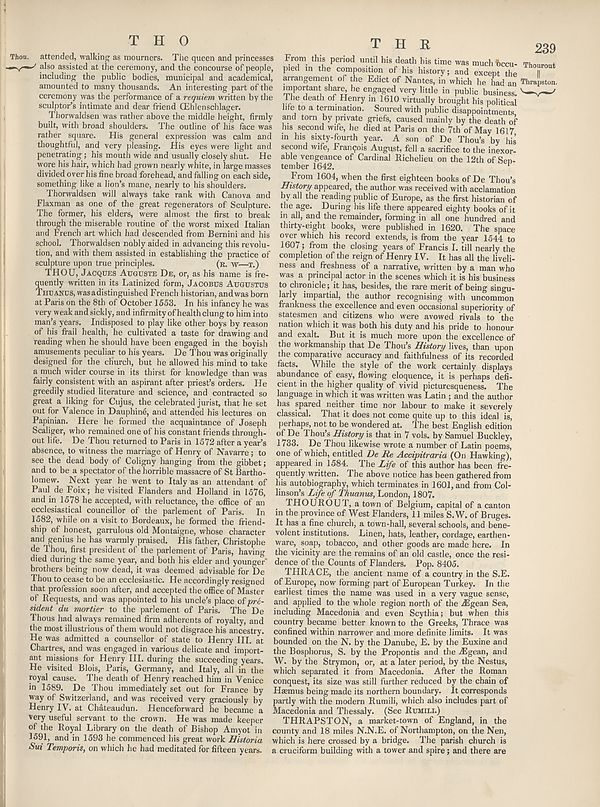
\includegraphics[width=0.85\textwidth]{../scans/page-0604-c50a825dd732.jpg}
\caption*{Source scan: \texttt{page-0604-c50a825dd732.jpg}}
\end{figure}

\end{document}
